\documentclass[border=1pt]{standalone}
\usepackage{mathptmx}  % Times text and math
\usepackage{circuitikz}
\usetikzlibrary{arrows.meta}
\ctikzset{bipoles/length=0.75cm, transistors/scale=0.9,
  inductors/coils=4, current/distance=.5, bipoles/diode/height=.32,
  bipoles/diode/width=.26}
\begin{document}
\fontsize{8}{9.6}\selectfont
% buck_vmode: control diagram, 1 layout unit = 1 cm (ieee-double)
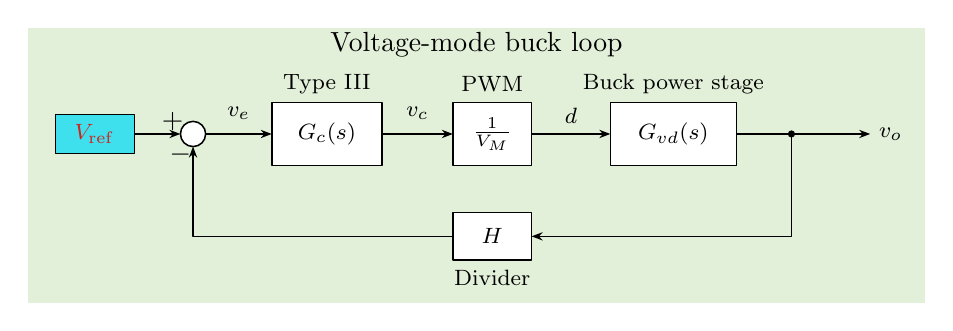
\begin{tikzpicture}[x=1cm, y=1cm, line width=0.55pt, line join=round]
% ---- regions (background) ----
\fill[fill={rgb,255:red,226;green,239;blue,217}] (-0.1,-2.15) rectangle (11.3,1.35);
\node[inner sep=0pt] at (5.6,1.14) {Voltage-mode buck loop};
% ---- links ----
\draw[-{Stealth[length=0.14cm]}] (1.25,0) -- (1.84,0);
\draw[-{Stealth[length=0.14cm]}] (2.16,0) -- (3,0);
\draw[-{Stealth[length=0.14cm]}] (4.4,0) -- (5.3,0);
\draw[-{Stealth[length=0.14cm]}] (6.3,0) -- (7.3,0);
\draw[-{Stealth[length=0.14cm]}] (8.9,0) -- (10.6,0);
\draw[-{Stealth[length=0.14cm]}] (9.6,0) -- (9.6,-1.3) -- (6.3,-1.3);
\draw[-{Stealth[length=0.14cm]}] (5.3,-1.3) -- (2,-1.3) -- (2,-0.16);
% ---- branch dots ----
\fill (9.6,0) circle (1.3pt);
% ---- ref (tag) ----
\filldraw[fill={rgb,255:red,63;green,224;blue,238}, draw={rgb,255:red,0;green,0;blue,0}, line width=0.33pt] (0.25,-0.25) rectangle (1.25,0.25);
% ---- e1 (sum) ----
\draw[fill=white] (2,0) circle (0.16cm);
% ---- gc (block) ----
\draw[fill=white] (3,-0.4) rectangle (4.4,0.4);
% ---- pwm (block) ----
\draw[fill=white] (5.3,-0.4) rectangle (6.3,0.4);
% ---- plant (block) ----
\draw[fill=white] (7.3,-0.4) rectangle (8.9,0.4);
% ---- h (block) ----
\draw[fill=white] (5.3,-1.6) rectangle (6.3,-1);
% ---- signs ----
\node[inner sep=0pt] at (1.74,0.16) {$+$};
\node[inner sep=0pt] at (1.84,-0.26) {$-$};
% ---- text ----
\node[inner sep=0pt, align=center, font=\fontsize{8}{9.6}\selectfont, text={rgb,255:red,208;green,35;blue,28}] at (0.75,0) {$V_{\mathrm{ref}}$};
\node[inner sep=0pt, align=center, font=\fontsize{8}{9.6}\selectfont] at (3.7,0) {$G_{c}(s)$};
\node[inner sep=0pt, align=center, font=\fontsize{8}{9.6}\selectfont] at (3.7,0.63) {Type III};
\node[inner sep=0pt, align=center, font=\fontsize{8}{9.6}\selectfont] at (5.8,0) {$\frac{1}{V_{M}}$};
\node[inner sep=0pt, align=center, font=\fontsize{8}{9.6}\selectfont] at (5.8,0.63) {PWM};
\node[inner sep=0pt, align=center, font=\fontsize{8}{9.6}\selectfont] at (8.1,0) {$G_{vd}(s)$};
\node[inner sep=0pt, align=center, font=\fontsize{8}{9.6}\selectfont] at (8.1,0.63) {Buck power stage};
\node[inner sep=0pt, align=center, font=\fontsize{8}{9.6}\selectfont] at (5.8,-1.3) {$H$};
\node[inner sep=0pt, align=center, font=\fontsize{8}{9.6}\selectfont] at (5.8,-1.83) {Divider};
\node[inner sep=0pt, align=center, font=\fontsize{8}{9.6}\selectfont] at (2.58,0.26) {$v_{e}$};
\node[inner sep=0pt, align=center, font=\fontsize{8}{9.6}\selectfont] at (4.85,0.26) {$v_{c}$};
\node[inner sep=0pt, align=center, font=\fontsize{8}{9.6}\selectfont] at (6.8,0.23) {$d$};
\node[inner sep=0pt, align=center, font=\fontsize{8}{9.6}\selectfont] at (10.86,0) {$v_{o}$};
\end{tikzpicture}
\end{document}
